\documentclass{standalone}
\usepackage{tikz}
\usepackage{ctex,siunitx}
\setCJKmainfont{Noto Serif CJK SC}
\usepackage{tkz-euclide}
\usepackage{amsmath}
\usetikzlibrary{patterns, calc}
\usetikzlibrary {decorations.pathmorphing, decorations.pathreplacing, decorations.shapes,}
\begin{document}
\small
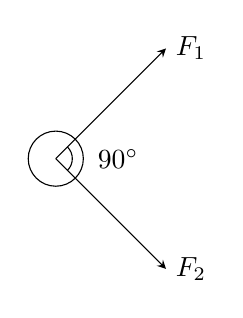
\begin{tikzpicture}[>=stealth,scale=0.7]
  \draw (0,0) circle (.5cm);
  \draw[->](0,0)--(2,2)node [right]{$F_1$};
  \draw[->](0,0)--(2,-2)node [right]{$F_2$};
  \draw (-45:0.3) arc (-45:45:.3)node [midway,right=2mm]{\ang{90}}; 
  % \draw (.3,0) arc (0:-45:.3);
\end{tikzpicture}
\end{document}